\documentclass[sigconf, anonymous, review]{acmart}

\usepackage{natbib}
\usepackage{algorithm}
\usepackage{algorithmic}
\usepackage{amsmath}
\usepackage{geometry}
\usepackage{verbatim}
\usepackage{tabularx}
\usepackage{graphicx}
\usepackage{amsfonts} % just for the indicator variable \mathbb{I}

\title{Elo-R Competition Rating System}
\author{Aram Ebtekar}
\date{December 2015 (revised on May 29, 2020)}

\begin{document}

\begin{abstract}
Skill estimation mechanisms, colloquially known as rating systems, play an important role in competitive sports and games. They provide a measure of player skill, which incentivizes competitive performances and enables balanced match-ups. In this paper, we present a novel Bayesian rating system for contests with many participants. It is widely applicable to competition formats with discrete ranked matches, such as online programming competitions, obstacle courses races, and video games. The system's simplicity allows us to prove theoretical bounds on its robustness and runtime. In addition, we show that it is \emph{incentive-compatible}: a player who seeks to maximize their rating will never want to underperform. Experimentally, the rating system surpasses existing systems in prediction accuracy, and computes faster than existing systems by up to an order of magnitude.
\end{abstract}

\maketitle


\section{Introduction}

% \begin{comment}
% Notes to self:
% - Should we do all-pairs ELO/Glicko per contest as a comparison?
%     - Performances where you do really well is amplified (\#1 is treated as O(n) wins where n is the number of competitors)
% - Can we prove the "aligned incentives" property? I.e. is a participant ever incentivized to lose?
%     - Can show that edits to past performance is monotonic w.r.t. to the edits

% Important points in introduction:
% - Rating systems are ad-hoc, preferences for algorithms based mostly on word-of-mouth and first movers.
% - Different domains use different systems (chess, football, etc --> elo based. team-based online games --> trueskill based or glicko based. coding contests --> ad-hoc, codeforces)
% - In general, the more complicated the rating system, the less adoptation.
% - Players overwhelmingly prefer the ability to understand and predict their own performance.
% - Rating systems are even used outside of sports: "Web-scale bayesian clickthrough
% rate prediction for sponsored search advertising in microsoft’s bing search
% engine" pits ads against each other in a TrueSkill-like fashion.
% - The goal of a rating system is two-fold: firstly to predict the results between players, but also equally as important is to give the players an easily interpretable proxy for their skill.

% Brief literature review:
% - In programming contests the actual scores do not matter much, the ranks give the most discriminative information
% - Talk about area of pairwise comparisons
%     - Paired comparisons assume static "ability" throughout time.
%     - First to look at time-varying paired comparisons was the glicko rating system
% - Glicko and Glicko 2:
%     - Improvement upon Elo in that the deviation was also explicitly modelled
%     - A drift parameter was also added to increase rating volatility over time
%     - This in turn increases the rating uncertainty since the uncertainty is updated from the volatility
%     - Flaws famously exploited in pokemon go, as rating gain is proportional to rating uncertainty
% - MOV Elo techniques:
%     - These not only take in ranking as input, but also "margin of victory". This is appropriate for more fine-grained contests where the same type of contest is played over and over again (e.g. tennis). For programming contests this is not as useful since the contest changes over and over again. Methods not directly applicable in our setting.
%     - Streamlines interface between rating system and contest type and for contest authors. More applicable to other domains. Goodhart's Law.
% - IRT rating system:
%     - Tasks of a contest are modelled explicitly. Allows for more fine grained predictions (such as the number of problems solved during a contest)
% - WHR (Who-Rating-History): a bayesian approach to ratings that takes into account time-varying strength
%     - Three types of rating sys: Static, Incremental, Decayed-History
%     - Our rating system is Incremental. Inferior in the following sense: suppose that there are two players (A & B) that only play against each other. Then A plays against established players. This gives information to B's rating, but incremental systems leave B's rating unchanged.
%     - This rating system doesnt seem to necessarily have a monotonicity property: the addition of a game could decrease the ratings of some of the players in the system who do not directly participate in the game? Players are not typically happy about this; good motivation for our second algorithm property
%     - Limit of large # of players guarantee a connectivity property
% - TrueSkill and TrueSkill 2: 
%     - Models games where medium sized teams of players play against each other
%     - Each user has some skill drawn from a distribution
%     - The performance on any given day is drawn from a distribution centred at the skill
%     - The performance of a team is the sum of team skills
%     - A parameter eps is defined so that performances with difference less than eps is counted as a tie.
%     - Trained through message passing
%     - Used in massive scale in Halo 2
%     - Convergence properties unclear, hard to proof stuff about it
%     - Normal vs logistics support.
%     - TrueSkill 2 takes into account further application-specific statistics
% - Trueskill Through Time:
%     - Similar to WHR in that a new game affects whole history. Does this suffer from non-monotonicity?
% - TrueSkill StPb:
%     - Improved on trueskill by adapting factor graph to handle ties in a principled way
%     - Nodes are added to the factor graph grouping teams that are tied
%     - Instead of summing team performances, non-linear team performance functions are explored
% - TeamSkill and TeamSkill Evolved:
%     - An ensemble learner that leverages TrueSkill, Elo, and Glicko to better predict ratings in the presence of "team chemistry" and non-equal team sizes.
%     - However only works when teams play together semi-consistently
% - Codeforces & leetcode:
%     - Generalized Elo system
%     - Heuristics to fight against inflation
%     - O(n^2) time.
%     - Used in leetcode as well, somewhat of an industry standard
%     - total website use at least 3 million users
% - Topcoder:
%     - More similar to glicko in the sense that each user has a rating deviation
%     - Successfully attacked by Forisek

% The Elo rating system assigns a quantitative measure of skill to each player. For example, an average player may be rated 1500, while a top player may exceed 2500. The scale is arbitrary, but can be used to rank players relative to one another. The odds of any one player winning against another may be estimated from the difference in their ratings. The famous Elo system, and variants such as Glicko \cite{G99}, provide useful formulas for updating ratings of players who compete 1v1 against one another, resulting in a winner and a loser. These algorithms have some nice properties: they are fairly simple, fast, and only modify the ratings of the two participating players.

% Now let's consider a general setting in which a typical contest has much more than two participants. An arbitrary number of players compete simultaneously at a task. Rather than producing just a winner and a loser, the contest ranks its participants 1st place, 2nd, 3rd, and so on. This description fits popular programming competition websites such as Codeforces \cite{Codeforces} and Topcoder \cite{Topcoder}, each of which has tens of thousands of rated members from across the globe. Each publishes its own rating system, but without much theoretical justification to accompany the derivations.

% We build Elo-MMR upon a more rigorous probabilistic model, mirroring the Bayesian development of the Glicko system. In doing so, we inherit its nice properties in practice, resolving known issues with the Codeforces and Topcoder systems. Compared with these systems, it achieves faster convergence and robustness against unusual performances. Issues specific to Codeforces than we improve upon are the overall spread of ratings, inter-division boundary artifacts, and inflation (TODO: cite, and quantify this with tests). An issue specific to Topcoder that we eliminate completely is non-monotonicity: simply put, there are cases in which improving a member's past performance would actually decrease their Topcoder rating, and vice-versa \cite{forivsektheoretical}.

% Furthermore, Elo-MMR retains simplicity and efficiency on par with the other systems. To demonstrate this, I provide a very efficient parallel implementation that can process the entire history of rated competitions hosted by Codeforces on a modest quad-core laptop within 30 minutes. It is implemented entirely within the safe subset of Rust using the Rayon crate; hence, the Rust compiler verifies that it contains no data races.

% This paper is organized as follows: in section 2, we develop a Bayesian model for the competitions. Rating updates are phrased as a latent skill estimation problem, which is naturally divided into two phases. Sections 3 and 4 describe each of these phases in turn, and supplement the derivations with some intuitive interpretations. Then in section 5, we discuss some ways to model uncertainty, in a manner analogous to the Glicko system. In section 6, we discuss some properties of the Elo-MMR system in comparison with the Codeforces and Topcoder systems. Finally, section 7 presents the conclusions of this work.
% \end{comment}

Competitions, in the form of sports, games, and examinations, have been with us since antiquity. Many competitions grade performances along a numerical scale, such as a score on a test or a completion time in a race. In the case of a college admissions exam or a track race, scores are standardized so that a given score on two different occasions carries the same meaning. However, in events that feature novelty, subjectivity, or close interaction, standardization is difficult. The Spartan Races, completed by millions of runners, feature a variety of obstacles placed on hiking trails around the world~\cite{Spartan}. Rock climbing, a sport to be added to the 2020 Olympics, likewise has routes set specifically for each competition. DanceSport, gymnastics, and figure skating competitions have a panel of judges who rank contestants against one another; these subjective scores are known to be noisy~\cite{DanceSport}. 
%Most board games feature considerable inter-player interaction.
In all these cases, scores can only be used to compare and rank participants at the same event. Players, spectators, and contest organizers who are interested in comparing players' skill levels across different competitions will need to aggregate the entire history of such rankings. A strong player, then, is one who consistently wins against weaker players. To quantify skill, we need a \textbf{rating system}.


Good rating systems are difficult to create, as they must balance several mutually constraining objectives. First and foremost, rating systems must be accurate, in that ratings provide useful predictors of contest outcomes. Second, the ratings must be efficient to compute: within video game applications, rating systems are predominantly used for matchmaking in massively multiplayer online games (such as Halo, CounterStrike, League of Legends, etc.)~\cite{HMG06, MCZ18, Y14}. These games have hundreds of millions of players playing tens of millions of games per day, necessitating certain latency and memory requirements for the rating system~\cite{AL09}. Third, rating systems must be \textbf{incentive-compatible}: a player's rating should never increase had they scored worse, and never decrease had they scored better.
%should never depend inversely on an absolute score. 
This is to prevent players from regretting a win, or from throwing matches to game the system. Rating systems that can be gamed often create disastrous consequences to player-base, potentially leading to the loss of players~\cite{pokemongo}. Finally, the ratings provided by the system must be human-interpretable: ratings are typically represented to players as a single number encapsulating their overall skill, and many players want to understand and predict how their performances affect their rating~\cite{G95}.

% Should we consider something about robustness, and about ratings not changing when a player doesn't compete? There are two things that these systems have in common. First, all of the these systems propagate changes forward in time, never backward. This is a strict requirement of the system in most cases, as users prefer their historical ratings to state fixed (even if it's possible to infer more accurate historical ratings from future matches). Such a property will be a requirement of our system as well.

Classically, rating systems were designed for two-player games. The famous Elo system~\cite{E61}, as well as its Bayesian successors Glicko and Glicko-2, have been widely applied to games such as Chess and Go~\cite{G95, G99, G12}. Both Glicko versions model each player's skill as a real random variable that evolves with time according to Brownian motion. Inference is done by entering these variables into the Bradley-Terry model~\cite{BT52}, which predicts probabilities of game outcomes. Glicko-2 refines the Glicko system by adding a rating volatility parameter. Unfortunately, Glicko-2 is known to be flawed in practice, potentially incentivizing players to lose in what's known as ``volatility farming''. In some cases, these attacks can inflate a user's rating \emph{several hundred points} above its natural value, producing ratings that are essentially impossible to beat via honest play. This was most notably exploited in the popular game of Pokemon Go~\cite{pokemongo}. See \Cref{sec:mono} for a discussion of this issue, as well as an application of this attack to the Topcoder rating system.

The family of Elo-like methods just described only utilize the binary outcome of a match. In settings where a scoring system provides a more fine-grained measure of match performance, Kovalchik~\cite{K20} has shown variants of Elo that are able to take advantage of score information. For competitions consisting of several set tasks, such as academic olympiads, Fori{\v{s}}ek~\cite{forivsektheoretical} developed a model in which each task gives a different ``response'' to the player: the total response then predicts match outcomes. However, such systems are often highly application-dependent and hard to calibrate.

%In terms of predictive power, the main disadvantage of Elo-like methods is that they are ``history-less'' and ``static''. That is, previous competitions of an individual are forgotten and summarized solely through a few per-user parameters. Consider an example where two groups of users compete within their own groups and never outside of their group. To compare the two groups, we may choose a representative user from each group to compete against each other. Given the results of this match, it should be possible to calibrate the ratings of all the users in the two groups accordingly. However, Elo-like methods only update the ratings of the two users participating in the match. Coulom~\cite{C08} exploit this observation by retaining the entire match history of a user, allowing for more accurate predictions. 

Though Elo-like systems are widely used in two-player settings, one needn't look far to find competitions that involve much more than two players. In response to the popularity of team-based games such as CounterStrike and Halo, many recent works focus on competitions that are between two teams~\cite{HLW06, CJ16, LCFHH18, GFYLWTFC20}. Another popular setting is many-player contests such as academic olympiads: notably, programming contest platforms such as Codeforces, Topcoder, and Kaggle~\cite{Codeforces, Topcoder, Kaggle}. As with the aforementioned Spartan races, a typical event attracts thousands of contestants. Programming contest platforms have seen exponential growth over the past decade, collectively boasting millions of users~\cite{KaggleMilestone}. As an example, Codeforces gained over 200K new users in 2019 alone~\cite{CFResults}.
%but they do not present efficient extensions for settings in which players are sorted into more than two, let alone thousands, of distinct places. For these cases, a rating system must take in a final ranking of the competitors, and produce a list of rating updates. 

In ``free-for-all'' settings, where $N$ players are ranked individually, the Bayesian Approximation Ranking (BAR) algorithm~\cite{WL11} models the competition as a series of $\binom N2$ independent two-player contests. In reality, of course, the pairwise match outcomes are far from independent. Thus, TrueSkill~\cite{HMG06} and its variants~\cite{NS10, DHMG07, MCZ18} model a player's performance during each contest as a single random variable. The overall rankings are assumed to reveal the total order among these hidden performance variables, with various methods used to model ties and teams. For a textbook treatment of these methods, see~\cite{Winn19}. These rating systems are efficient in practice, successfully rating userbases that number well into the millions (the Halo series, for example, has over 60 million sales since 2001~\cite{Halo}).

The main disadvantage of TrueSkill is its complexity: originally developed by Microsoft for the popular Halo video game, TrueSkill performs approximate belief propagation, which consists of message passing on a factor graph, iterated until convergence. Aside from being less human-interpretable, this complexity means that, to our knowledge, there are no proofs of key properties such as runtime and incentive-compatibility. Even when these properties are discussed~\cite{MCZ18}, no rigorous justification is provided. In addition, we are not aware of any work that extends TrueSkill to non-Gaussian performance models, which might be desirable to limit the influence of outlier performances (see \Cref{sec:robust}).

It might be for these reasons that popular platforms such as Codeforces and Topcoder opted for their own custom rating systems. These systems are not published in academia and do not come with Bayesian justifications. However, they retain the formulaic simplicity of Elo and Glicko, extending them to settings with much more than two players. The Codeforces system includes ad hoc heuristics to distinguish top players, while curbing rampant inflation. Topcoder's formulas are more principled from a statistical perspective; however, it has a volatility parameter similar to Glicko-2, and hence suffers from similar exploits~\cite{forivsektheoretical}. Despite their flaws, these systems have been in place for over a decade, and have more recently gained adoption by additional platforms such as CodeChef and LeetCode~\cite{LeetCode, CodeChef}.


\paragraph{Our contributions} 
In this paper, we describe the Elo-MMR rating system, obtained by a principled approximation of a Bayesian model similar to Glicko and TrueSkill. It is fast, embarrassingly parallel, and makes accurate predictions. Most interesting of all, its simplicity allows us to rigorously analyze its properties: the ``MMR'' in the name stands for ``Massive'', ``Monotonic'', and ``Robust''. ``Massive'' means that it supports any number of players with a runtime that scales linearly; ``monotonic'' is a synonym for incentive-compatible, ensuring that a rating-maximizing player always wants to perform well; ``robust'' means that rating changes are bounded, with the bound being smaller for more consistent players than for volatile players. Robustness turns out to be a natural byproduct of accurately modeling performances with heavy-tailed distributions, such as the logistic. TrueSkill is believed to satisfy the first two properties, albeit without proof, but fails robustness. Codeforces only satisfies incentive-compatibility, and Topcoder only satisfies robustness.

Experimentally, we show that Elo-MMR achieves state-of-the-art performance in terms of both prediction accuracy and runtime on industry datasets. In particular, we process the entire Codeforces database of over 300K rated users and 1000 contests in well under a minute, beating the existing Codeforces system by an order of magnitude while improving upon its accuracy. Furthermore, we show that the well-known Topcoder system is severely vulnerable to volatility farming, whereas Elo-MMR is immune to such attacks. A difficulty we faced was the scarcity of efficient open-source rating system implementations. In an effort to aid researchers and practitioners alike, we provide open-source implementations of all rating systems, dataset mining, and additional processing used in our experiments at {\tt\url{https://github.com/EbTech/Elo-MMR}}.

\paragraph{Organization}
In \Cref{sec:bayes_model}, we formalize the details of our Bayesian model. We then show how to estimate player skill under this model in \Cref{sec:main-alg}, and develop some intuitions of the resulting formulas. As a further refinement, \Cref{sec:skill-drift} models skill evolutions from players training or atrophying between competitions. This modeling is quite tricky as we choose to retain players' momentum while preserving incentive-compatibility. While our modeling and derivations occupy multiple sections, the system itself is succinctly presented in \Cref{alg:main,alg:diffuse,alg:update}. In \Cref{sec:properties}, we perform a volatility farming attack on the Topcoder system and prove that, in contrast, Elo-MMR satisfies several salient properties, the most critical of which is incentive-compatibility. Finally, in \Cref{sec:experiments}, we present experimental evaluations, showing improvements over industry standards in both accuracy and speed. An extended version of this paper, with additional proofs and experiments, can be found at {\tt\url{https://arxiv.org/abs/2101.00400}}.

\section{Bayesian Model}

Now we describe the setting formally. A series of competitive \textbf{rounds}, indexed by $t=1,2,3,\ldots$, take place sequentially in time. The participants of a round $t$ are a subset of all the \textbf{players}, which are indexed by $i$. At time $t$, player $i$ has latent \textbf{skill} $s_{i,t}$, which we seek to estimate from a history of observable \textbf{evidence} $e_1,\ldots,e_t$ produced by the rounds $1,\ldots,t$.

In Bayesian fashion, we start with a prior belief distribution on $s_{i,t}$ immediately preceding round $t$, taking into account all of the rounds $1,2,\ldots,t-1$. Our main task is to combine the prior belief with the evidence $e_t$ to obtain a posterior belief. This will serve as the basis for a post-round \textbf{rating}, defined to be the \textbf{maximum a posteriori} (MAP) estimate of $s_{i,t}$. That is,

\begin{align*}
r_{i,t} &= \arg\max_{s_{i,t}} f(s_{i,t} \mid e_1,\ldots,e_t) \\
&= \arg\max_{s_{i,t}} f(s_{i,t} \mid e_1,\ldots,e_{t-1}) \Pr(e_t \mid s_{i,t})
\end{align*}

where $f(s_{i,t} \mid e_1,\ldots,e_t)$ is the probability density function (p.d.f.) corresponding to our posterior belief on player $i$'s latent skill given the history of evidence. Here we used Bayes' rule to write the posterior p.d.f. as proportional to the product of the prior p.d.f. and the evidence probability.

Let's simplify the notation. Since the pre-round evidence $e_1,\ldots,e_{t-1}$ is common to both the prior and posterior beliefs, we treat them as understood and explicitly write only the new evidence $e_t$. This leaves $t$ as the only round subscript, so we omit that as well. With these changes, the post-round rating can be re-written more simply as

\[r_i = \arg\max_{s_i} f(s_i \mid e) = \arg\max_{s_i} f(s_i) \Pr(e \mid s_i)\]

We assume the evidence $e$ is produced from each round in the following generative fashion: each participant randomly draws their performance $p_i$ in the round independently from a logistic distribution centered at $s_i$, with a variance $\gamma_i^2$ that may depend on characteristics of the round $t$ (whose subscript we continue to omit) and player $i$.

While the variables $s_i$ and $p_i$ are hidden, we assume that player $i$ outranks player $j$ (written $i \succ j$) in the round if, and only if, $p_i > p_j$, and that we observe the complete relative rankings. In other words, the observable evidence $e$ consists of a total order on the set of participants.

Due to this important modeling assumption, the method is best-suited for competitions in which the most pertinent information is round rankings. Note that, in the programming contest setting, this means we discard specific information about player scores, which are difficult to model and depend heavily on the specifics of the problem set. This method would be ill-suited to model, for instance, track races, where a runner's absolute time is more informative than relative rankings. On the other hand, it may be very well-suited to obstacle-course races, if each round consists of novel obstacles that make the absolute times hard to interpret.

Strictly speaking, ties have probability zero of occurring in our model. Assuming that ties are relatively infrequent in programming contests, they can be handled with a special modification that we'll describe later, essentially treating them as half a win and half a loss.

\begin{center} 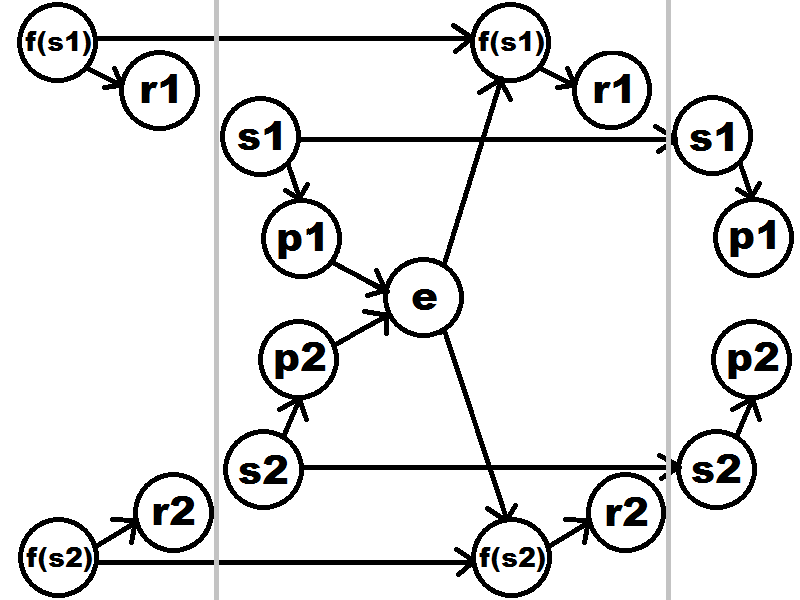
\includegraphics[scale=0.35]{../images/HMMlabeled.png} \end{center}

In order to absorb $e$ into our posterior, a few approximations are in order. First, we assume the number of participants is so large that we are able to compute the performances exactly. Mathematically, this means $\Pr(e \mid p_i)$ is proportional to a delta ``function" concentrated at the correct value of $p_i$. Hence, using Bayes' rule again,

\begin{align*}
f(s_i\mid e)
&\propto f(s_i)\Pr(e\mid s_i)
\\&= f(s_i)\int \Pr(e\mid p_i)f(p_i\mid s_i)\,dp_i
\\&\propto f(s_i)f(p_i\mid s_i)
\end{align*}

where the constants of proportionality depend on $e$ but not on $s_i$.

This suggests a natural two-phase update algorithm for each player $i$. In phase one, we estimate the MAP of $p_i$ given $e$. This estimate has very low error in the limit of very many participants, so we can take the MAP of $p_i$ to be its true value. In phase two, we update the posterior according to the above expression, and compute the new rating $r_i$ as the MAP of $s_i$ given $e$.

Note that, since the $p_i$ are assumed to be computed exactly, there is never a reason to retroactively update past estimates of performance. It follows that a round's non-participating players have posterior skill distribution identical to their prior; in particular, their ratings do not change.
\subsection{Performance estimation}
\label{sec:performance}

In this section, we describe the first phase of Elo-MMR. For notational convenience, we assume all probability expressions to be conditioned on the \textbf{prior context} $P_{i,< t}$, and omit the subscript $t$.

Our prior belief on each player's skill $S_i$ implies a prior distribution on $P_i$. Let's denote its probability density function (pdf) by
\begin{equation}
\label{eq:perf-prior} 
f_i(p) := \Pr(P_i = p) = \int \pi_i(s) \Pr(P_i = p \mid S_i=s) \,\mathrm{d}s,
\end{equation}
where $\pi_i(s)$ was defined in \Cref{eq:pi-s}. Let
\[F_i(p) := \Pr(P_i\le p) = \int_{-\infty}^p f_i(x) \,\dx,\]
be the corresponding cumulative distribution function (cdf). For the purpose of analysis, we'll also define the following ``loss'', ``draw'', and ``victory'' functions:
\begin{align*}
l_i(p) &:= \ddp\ln(1-F_i(p)) = \frac{-f_i(p)}{1 - F_i(p)},
\\d_i(p) &:= \ddp\ln f_i(p) = \frac{f'_i(p)}{f_i(p)},
\\v_i(p) &:= \ddp\ln F_i(p) = \frac{f_i(p)}{F_i(p)}.
\end{align*}

Evidently, $l_i(p) < 0 < v_i(p)$. Now we define what it means for the deviation $P_i - S_i$ to be log-concave.
\begin{definition}
\label{def:log-concave}
An absolutely continuous random variable on a convex domain is \textbf{log-concave} if its probability density function $f$ is positive on its domain and satisfies
\[f(\theta x + (1-\theta) y) > f(x)^\theta f(y)^{1-\theta},\;\forall\theta\in(0,1),x\neq y.\]
\end{definition}

Log-concave distributions appear widely, and include the Gaussian and logistic distributions used in Glicko, TrueSkill, and many others. We'll see inductively that our prior $\pi_i$ is log-concave at every round. Since log-concave densities are closed under convolution~\cite{concave}, the independent sum $P_i=S_i+(P_i-S_i)$ is also log-concave. Log-concavity is made very convenient by the following lemma, proved in the extended version of this paper:
\begin{lemma}
\label{lem:decrease}
If $f_i$ is continuously differentiable and log-concave, then the functions $l_i,d_i,v_i$ are continuous, strictly decreasing, and
\[l_i(p) < d_i(p) < v_i(p) \text{ for all }p.\]
\end{lemma}

For the remainder of this section, we fix the analysis with respect to some player $i$. As argued in \Cref{sec:bayes_model}, $P_i$ concentrates very narrowly in the posterior. Hence, we can estimate $P_i$ by its MAP, choosing $p$ so as to maximize:
\[\Pr(P_i=p\mid E^L_i,E^W_i) \propto f_i(p) \Pr(E^L_i,E^W_i\mid P_i=p).\]

Define $j\succ i$, $j\prec i$, $j\sim i$ as shorthand for $j\in E^L_i$, $j\in E^W_i$, $j\in \mathcal P\setminus (E^L_i\cup E^W_i)$ (that is, $P_j>P_i$, $P_j<P_i$, $P_j=P_i$), respectively. The following theorem yields our MAP estimate:
\begin{theorem}
\label{thm:uniq-max}
Suppose that for all $j$, $f_j$ is continuously differentiable and log-concave. Then the unique maximizer of $\Pr(P_i=p\mid E^L_i,E^W_i)$ is given by the unique zero of
\[Q_i(p) := \sum_{j \succ i} l_j(p) + \sum_{j \sim i} d_j(p) + \sum_{j \prec i} v_j(p).\]
\end{theorem}
The proof appears in the extended version of this paper. Intuitively, we're saying that the performance is the balance point between appropriately weighted wins, draws, and losses. Let's look at two specializations of our general model, to serve as running examples in this paper.

\paragraph{Gaussian performance model}
If both $S_j$ and $P_j-S_j$ are assumed to be Gaussian with known means and variances, then their independent sum $P_j$ will also be a known Gaussian. It is analytic and log-concave, so \Cref{thm:uniq-max} applies.

We substitute the well-known Gaussian pdf and cdf for $f_j$ and $F_j$, respectively. A simple binary search, or faster numerical techniques such as the Illinois algorithm or Newton's method, can be employed to solve for the unique zero of $Q_i$.

\begin{figure}
    \centering
    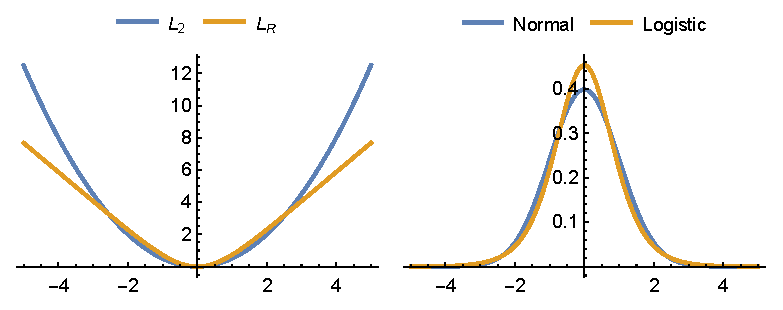
\includegraphics[width=1.05\columnwidth]{images/l2-lr-plot.eps}
    \caption{$L_2$ versus $L_R$ for typical values (left). Gaussian versus logistic probability density functions (right).}
    \label{fig:l2-lr-plot}
\end{figure}

\paragraph{Logistic performance model}
Now we assume the performance deviation $P_j-S_j$ has a logistic distribution with mean 0 and variance $\beta^2$. In general, the rating system administrator is free to set $\beta$ differently for each contest. Since shorter contests tend to be more variable, one reasonable choice might be to make $1/\beta^2$ proportional to the contest duration.

Given the mean and variance of the skill prior, the independent sum $P_j = S_j + (P_j-S_j)$ would have the same mean, and a variance that's increased by $\beta^2$. Unfortunately, we'll see that the logistic performance model implies a form of skill prior from which it's tough to extract a mean and variance. Even if we could, the sum does not yield a simple distribution.

For experienced players, we expect $S_j$ to contribute much less variance than $P_j-S_j$; thus, in our heuristic approximation, we take $P_j$ to have the same form of distribution as the latter. That is, we take $P_j$ to be logistic, centered at the prior rating $\mu^\pi_j = \argmax \pi_j$, with variance $\delta_j^2 = \sigma_j^2 + \beta^2$, where $\sigma_j$ will be given by \Cref{eq:variance}. This distribution is analytic and log-concave, so the same methods based on \Cref{thm:uniq-max} apply. 
Define the scale parameter $\bar\delta_j := \frac{\sqrt{3}}{\pi} \delta_j$. A logistic distribution with variance $\delta_j^2$ has cdf and pdf:
\begin{align*}
F_j(x) &= \frac { 1 } { 1 + e^{-(x-\mu^\pi_j)/\bar\delta_j} }
= \frac 12 \left(1 + \tanh\frac{x-\mu^\pi_j}{2\bar\delta_j} \right),
\\f_j(x) &= \frac { e^{(x-\mu^\pi_j)/\bar\delta_j} } { \bar\delta_j\left( 1 + e^{(x-\mu^\pi_j)/\bar\delta_j} \right)^2}
= \frac { 1 } { 4\bar\delta_j} \sech^2\frac{x-\mu^\pi_j}{2\bar\delta_j}.
\end{align*}

The logistic distribution satisfies two very convenient relations:
\begin{align*}
F'_j(x) = f_j(x) &= F_j(x) (1 - F_j(x)) / \bar\delta_j,
\\f'_j(x) &= f_j(x) (1 - 2F_j(x)) / \bar\delta_j,
\end{align*}
from which it follows that
\[d_j(p)
= \frac{1 - 2F_j(p)}{\bar\delta}
= \frac{-F_j(p)}{\bar\delta} + \frac{1 - F_j(p)}{\bar\delta}
= l_j(p) + v_j(p).\]

In other words, a tie counts as the sum of a win and a loss. This can be compared to the approach (used in Elo, Glicko, BAR, Topcoder, and Codeforces) of treating each tie as half a win plus half a loss.\footnote{Elo-MMR, too, can be modified to split ties into half win plus half loss. It's easy to check that \Cref{lem:decrease} still holds if $d_j(p)$ is replaced by
$w_l l_j(p) + w_v v_j(p)$
for some $w_l,w_v\in [0,1]$ with $|w_l-w_v|<1$.
In particular, we can set $w_l=w_v=0.5$. The results in \Cref{sec:properties} won't be altered by this change.}

Finally, putting everything together:
\[Q_i(p) = \sum_{j \succeq i} l_j(p) + \sum_{j \preceq i} v_j(p)
= \sum_{j \succeq i} \frac{-F_j(p)}{\bar\delta_j} + \sum_{j \preceq i} \frac{1 - F_j(p)}{\bar\delta_j}.\]
Our estimate for $P_i$ is the zero of this expression. The terms on the right correspond to probabilities of winning and losing against each player $j$, weighted by $1/\bar\delta_j$. Accordingly, we can interpret $\sum_{j\in \cP} (1-F_j(p))/\bar\delta_j$ as a weighted expected rank of a player whose performance is $p$. Similar to the performance computations in Codeforces and Topcoder, $P_i$ can thus be viewed as the performance level at which one's expected rank would equal $i$'s actual rank.




\section{Belief Update}

With $p_i$ in hand, we are ready for the second phase of the update! Recall that we seek to maximize

\[f(s_i\mid e) \propto f(s_i)f(p_i\mid s_i)\]

Ignoring for now the distinction between the posterior at round $t-1$ and the prior at round $t$ (we'll come back to this in the next section), we see that each round multiplies our belief p.d.f. by a logistic factor and a normalizing constant. Thus, our belief will always consist of a product of p.d.f.s.

Let's be a tad more general here and allow the belief to be any normalized product of normal and logistic p.d.f.s. The normal p.d.f.s can be composed into a single normal with mean and variance $(\mu_0, \tau_0^2)$. Let $R_i$ be the set of rounds in which player $i$ has participated, each contributing a logistic factor with parameters $(\mu_k, \tau_k^2)$ for $k\in R_i\cap \{1,\ldots,t\}$. Naturally, the new factor from round $t$ will have $\mu_t = p_{i,t}$ and $\tau_t = \gamma_{i,t}$. The other factors also satisfy $\mu_k = p_{i,k}$ but, as we'll see in the next section, $\tau_k$ increases with time and will exceed $\gamma_{i,k}$ in general. Again defining $\bar\tau_k = \frac{\sqrt{12}}{\pi} \tau_k$,

\[
f(s_i\mid e)
\propto e^{-(s_i-\mu_0)^2/\tau_0^2} \prod_{k\ge 1} \frac { 1 } { \cosh^2\frac{s_i-\mu_k} {\bar\tau_k} }
\]

Hence, there exists a constant $C$ such that

\[C - \frac 1 2 \ln f(s_i \mid e) = \frac{(s_i-\mu_0)^2}{2\tau_0^2} + \sum_{k\ge 1} \ln\left( \cosh\frac{s_i-\mu_k}{\bar\tau_k} \right)\]

Maximizing $f(s_i\mid e)$ amounts to minimizing this expression, so let's differentiate it w.r.t. $s_i$ and set the result to zero:

\[
0 = \frac{s_i-\mu_0}{\tau_0^2} + \sum_{k\ge 1} \frac{1}{\bar\tau_k} \tanh \frac {s_i-\mu_k} {\bar\tau_k}
\]

Similar to the performance computation in the previous section, here we have a monotonic function of $s_i$. To compute the post-round rating $r_i = \arg\max_{s_i} f(s_i \mid e)$, we may use binary search or Newton's method.

This time, the intuitive interpretation comes from the minimization objective that we differentiated. It has one term corresponding to each p.d.f. factor. The normal p.d.f. becomes a familiar $L^2$ penalty that pushes $s_i$ towards $\mu_0$. The logistic p.d.f.s are more interesting: they too become penalties that push $s_i$ towards $\mu_k$; however, instead of a simple squared error, each of these terms is a logarithm of a hyperbolic cosine!

At small scales (that is, when $|s_i-\mu_k| \ll \tau_k$), it acts like an $L^2$ penalty. However, at large scales (when $|s_i-\mu_k| \gg \tau_k$), it acts like an $L^1$ penalty! It's well-known that minimizing a sum of $L^2$ terms pushes the argument towards a weighted mean, while minimizing a sum of $L^1$ terms pushes the argument towards a weighted median.

The net result of these penalties is that $r_i$ acts like a mean of the historical performances $\mu_k = p_{i,k}$: it's easily checked that

\[r_i = \frac{\sum_k w_k\mu_k}{\sum_k w_k} \text{ where } w_0 = \frac{1}{\tau_0^2} \text{ and }
w_k = \frac{1}{\bar\tau_k(r_i-\mu_k)}\tanh\frac{r_i-\mu_k}{\bar\tau_k} \text{ for }k\ge 1.\]

$w_k$ is close to $1/\bar\tau_k^2$ for typical performances but vanishes for extreme outliers, making our rating algorithm robust to performances that are far below or above the usual. This robustness is due to the thicker tails of the logistic distribution, compared to the normal. Empirically, contest performances have indeed been seen to have thick tails, more like the logistic than the normal (TODO citation).

Note that when the weights are fixed, as in the $L^2$ case, it's possible to compute the posterior rating as a function of only the prior rating, prior weight, and the current round's performance and weight. This is no longer possible when using $L^1$ or $\ln\cosh$ penalties. Naively, it appears this method must remember the entire history of past performances: certainly, the latest rating alone is insufficient.

Luckily, it's possible to sustain negligible loss of precision while retaining only a bounded history length per player, thus keeping the time and memory overhead to within a constant factor. The exact means by which this is achieved depends on the noising method used, a matter we'll discuss later. For now, note that the $\tanh$ function behaves like the identity in the limit of large $\tau_k$. Hence, logistic factors with sufficiently large $\tau_k$ will come to resemble normal factors, which combine nicely.

As a final matter, we estimate the variance $\sigma_i^2$ of the posterior distribution on $s_i$. While this is intractable for general products of p.d.f.s, we take advantage of our observation that logistic factors behave in the limit like normal factors. Thus, we make an approximation based on a formula that holds for products of normal p.d.f.s:

\[\frac{1}{\bar\sigma_i^2} = \frac{1}{\tau_0^2} + \sum_k \frac{1}{\bar\tau_k^2}\]

\section{Priors}

So far, we've shown how to go from prior belief to posterior belief in any given round. But how do we get priors? For first-time contestants, we answer this question with a ``newbie prior". For existing contestants, we must derive the new round's prior $f(s_{i,t} \mid e_1,\ldots,e_{t-1})$ from the previous round's posterior $f(s_{i,t-1} \mid e_1,\ldots,e_{t-1})$. These differ because a player whose skill evolves over time will generally have $s_{i,t} \ne s_{i,t-1}$.

The newbie prior has a great impact on the time it takes the rating distribution for a population of players to converge. Implicit in our argument that $p_i$ can be computed precisely, was an assumption that the belief distributions are accurate prior to the round. In order for this to be true, the newbie prior should approximately reflect the skill distribution among newcomers, particularly when the system is initialized. To the extent that it does not, the $p_i$'s may be inaccurate for some waiting period, until the population's rating distribution converges.

For Codeforces, I chose a normal prior with mean 1500 and standard deviation 350. The normal's thin tails discourage the granting of extreme ratings until sufficient evidence is gathered to justify it. To more strongly discourage premature assignment of extreme ratings, a smaller standard deviation can be used, albeit potentially at the expense of convergence speed.

Now we consider players who have competed before. Since we deal with one player at a time, in this section we omit the player subscript $i$ but keep the round subscripts $t$:

\[
f(s_t \mid p_1,\ldots,p_{t-1})
= \int_{s_{t-1}} f(s_t \mid s_{t-1}) \, f(s_{t-1} \mid p_1,\ldots,p_{t-1}) \,ds_{t-1}
\]

That is, the new prior is an weighted integral of the old posterior. The weight $f(s_t \mid s_{t-1})$ models the evolution of a player; its form should depend on what characteristics are desired of the rating system. Typically, we don't want to adjust the center $r$ of a player's skill distribution, but we should increase the variance $\sigma^2$ to account for the fact that a player may have improved or worsened during the time in which we haven't seen them compete. Thus, we model $s_t$ as a random draw from a distribution (perhaps normal or logistic) with mean $s_{t-1}$ and variance $\eta_t^2$.

There are different ways to set the noise magnitude $\eta_t^2$. If we set it to be proportional to the time elapsed between the two rounds, the player's variance would increase at a constant rate, as if it were slowly and randomly perturbed by a process of Brownian motion. In this model, a long-inactive player's skill has to potential to change drastically upon their return. In a system that implements such Brownian noise, if we report the lower-bound estimate $r-2\sigma$ instead of $r$, we would find that ratings gradually decay, favoring active players and gradually diminishing inactive ones.

For Codeforces, we prefer to preserve the ratings of inactive players. Furthermore, we consider it likely that players who compete frequently will develop much faster than those who are inactive. Thus, it makes sense to increase uncertainty on a per-round basis rather than on a continuous per-time basis. So we use zero noise before rounds where the player is absent, while $\sigma^2$ is increased by a constant $\eta^2$ before each round in which the player is present. Post-round, their $\sigma^2$ is decreased as a function of the performance uncertainty, which I set to a constant $\bar\gamma = 250$ (though one might consider smaller $\gamma$ for longer contests, which are likely to be more informative). Over a large number of rounds, this process will eventually approach the limit $\sigma^*$ given by the fixpoint equation:

\begin{align*}
\frac{1}{\sigma^{*2}} &= \frac{1}{\sigma^{*2} + \eta^2} + \frac{1}{\gamma^2}
\\ \text{Setting }\bar\sigma^*=100\text{, I derived }\bar\eta^2 &= \frac{1}{1/\bar\sigma^{*2} - 1/\bar\gamma^2} - \bar\sigma^{*2} \approx 43.64^2
\end{align*}

Note that if the newbie uncertainty is set to $\sigma^*$, we obtain a system in which the inter-round noise $\eta$ exactly compensates for the round information $\gamma$, and so $\sigma$ stays constant, similar to traditional Elo. Setting the newbie uncertainty above $\sigma^*$ causes the uncertainty to decrease with each participation, similar to Glicko. I like to report $r-2(\bar\sigma-\bar\sigma^*)$ as a player's public rating. In the absence of time-based Brownian noise, this doesn't cause rating decay; instead, its effect is to penalize new members: their published rating is about $r - 208$ after their first contest, $r - 120$ after their second, and so on, the penalty approaching $0$. Since players start with a low published rating instead of an average one, even middle ratings can be considered an achievement, giving beginners a goal to strive for. 

\subsection{Approximate Noising}

Regardless of how and when the magnitude of noise is decided, we have an intractable integral to evaluate. Indeed, this is where we'll have the most difficulty justifying our approximations. Future research may find improvements in this aspect of the rating system.

What can be said about the integral? Well, if the inter-round noise is i.i.d. with zero mean, then the new prior should have the same mean (hence, likely a similar mode) and its variance should be increased by $\eta^2$. Furthermore, for computational ease and human-interpretability, it would be nice if the new prior remains a product of the same p.d.f.s as the posterior, only with each of their variances increased. Altogether, I came up with four methods that satisfy these properties; their pros and cons are summarized in Section 6.2.

The first and simplest method is also the only one that makes the player ratings (with accompanying uncertainties) a Markov state: that is, no history of past performances is kept. Every time a new rating $(r_i,\sigma_i^2)$ is computed, the posterior is approximated by a normal distribution with the same parameters. In this case, the effect of adding a normal $(0,\eta^2)$ noise is simple: the next round's prior becomes another normal, with parameters $(r_i,\,\sigma_i^2+\eta^2)$.

\begin{algorithm}
	\caption{$init()$}
	\label{alg:init}
	\begin{algorithmic}
		\STATE $\sigma^* := 100$
		\STATE $\gamma := 250$
		\STATE $\eta := \sqrt{1 / \left( 1/\sigma^{*2} - 1/\gamma^2 \right) - \sigma^{*2}}$
		\FORALL{players $i$}
		\STATE $r_i := 1500$
		\STATE $\sigma_i := 350$
		\ENDFOR
	\end{algorithmic}
\end{algorithm}

\begin{algorithm}
	\caption{$update()$}
	\label{alg:update}
	\begin{algorithmic}
		\FORALL{round participants $i$ in parallel}
		\STATE $r'_i := r_i$
		\STATE $\sigma_i := \sqrt{\sigma_i^2 + \eta^2}$
		\STATE $\delta_i := \sqrt{\sigma_i^2 + \gamma^2}$
		\STATE Make $r'_i,\delta_i$ accessible to all threads in the next loop
		\ENDFOR
		\FORALL{round participants $i$ in parallel}
		\STATE $p_i := $ SOLVE $\sum_{j\preceq i}\frac{1}{\delta_j}\left( \tanh\frac {p_i - r'_j} {\delta_j} - 1 \right) + \sum_{j\succeq i}\frac{1}{\delta_j}\left( \tanh\frac {p_i - r'_j} {\delta_j} + 1 \right) = 0$
		\STATE $r_i := $ SOLVE $\frac{r_i-r'_i}{\sigma_i^2} + \frac{1}{\gamma} \tanh \frac {r_i-p_i} {\gamma} = 0$
		\STATE $\sigma_i := 1 / \sqrt{1/\sigma_i^2 + 1/\gamma^2}$
		\ENDFOR
	\end{algorithmic}
\end{algorithm}

The parameter and belief initializations are summarized in Algorithm \ref{alg:init}, while the actual Elo-R update is summarized in Algorithm \ref{alg:update}. Upper-bars are not drawn, but should be taken as implicit on all variances aside from the normal prior. By working with these modified variances, the algorithm avoids needing to compute the factor $\frac{\sqrt{12}}{\pi}$.

The runtime analysis is straightforward. Suppose the round in question has $N$ participants, and the equations are solved to a precision of $\epsilon$ using binary search. Then it costs $O(N\log\frac 1\epsilon)$ time to solve for each $p_i$. Since this step dominates the computation, the total work done to process one round is $O(N^2\log\frac 1\epsilon)$. The logarithmic factor can be reduced with better equation-solving procedures, such as Newton's method. The round update is highly parallel, so its parallel span is roughly the total work divided by the number of processors.

\subsection{Alternative Noising Methods (TODO: everything from here onwards needs serious rewriting. Please stop reading!)}

Now we explore extensions in which the ratings and uncertainties alone are not Markov states: that is, we maintain each belief distribution as a product of p.d.f.s. The variance of such a product distribution is intractable, so we take it to be given by the formula at the end of section 4. If we simply multiply the variance of each factor by the same value $1 + \frac{\eta^2}{\sigma^2}$, this formula multiplies the overall variance by the same amount, yielding exactly the desired variance $\sigma^2+\eta^2$.

Heuristically speaking, we might justify this constant multiplication method by appealing to the limit of normal priors: by holding constant the ratio of weights between normal contributions, we hold the mean (and mode) of the whole distribution constant. Intuitively, if we think of each factor as a ``measurement" of the current skill $s_{i,t}$, then the noise operation simply reduces our confidence in outdated measurements.

As promised in the previous section, now we see that each $\tau_k$ in the belief distribution will increase exponentially with additional rounds. Pretty soon, any plausible skill level $s_i$ will fall squarely within the regime where $|s_i-\mu_k| \ll \tau_k$. As a result, the older logistic factors can safely be absorbed into the normal factor.

However, the same observation reveals a flaw with the constant multiplication method: as $\tau_k$ increases, outliers eventually become non-outliers, pulling $r$ towards the mean of old performances! In other words, we discount the weight of outlier performances more slowly than typical ones, until the outlier-specific weight reduction is negated entirely. This has two undesirable consequences: (1) the posterior mode $r$, which is the player's rating, changes during inactivity; (2) in the long term, outliers have equal weight to typical performances.

Arguably a better way to add noise would be to reduce the weight of each factor equally in all cases, not just in the normal limit. In essence, we gradually ``freeze in" the outlier weight reduction, based on how far each $\mu_k$ is from the current $r$.

To be mathematically precise, we binary search for the unique weight reduction factor $\kappa>1$ such that, if $\tau'_0=\kappa\tau_0$, and each $\tau'_k$ is the unique solution to

\[
\frac{1}{\bar\tau'_k} \tanh \frac {r-\mu_k} {\bar\tau'_k}
= \frac{1}{\kappa^2\bar\tau_k} \tanh \frac {r-\mu_k} {\bar\tau_k},\qquad
\text{then} \quad \frac{1}{\bar\sigma_i^2 + \bar\eta^2}
= \frac{1}{\tau_0'^2} + \sum_k \frac{1}{\bar\tau_k'^2}.
\]

By summing the left-hand side of the first equation over all $k$, we see that the mode doesn't change when we replace each $\tau_k$ by $\tau'_k$. With this noising procedure, the Elo-R weighted average takes an interesting form: outliers maintain a reduced weight for all time, but the \textit{extent} to which their weight is reduced is dependent on how much of an outlier they were during the period in which they were ``fresh". For instance, an outlier can gain non-outlier status if subsequent performances reinforce it. However, it's impossible to ``re-activate" an outlier from ancient history. This makes sense, since old flukes likely have nothing to do with new rapid skill changes. The downside of this noising method is that it violates rating system monotonicity, in certain cases.

The parameter and belief initializations are summarized in Algorithm \ref{alg:init2}, while the actual Elo-R update is summarized in Algorithm \ref{alg:update2}. As before, upper-bars are not drawn. The weights $w_{i,k}$ are given by the formula in section 4; $w'_{i,k}$ is derived by replacing $\tau_{i,k}$ with $\tau'_{i,k}$.

The time complexity now has an additional significant term: if $M$ rounds of history are kept, then it costs $O(M\log^2\frac 1\epsilon)$ to apply the noising procedure to each player. Altogether, the total work done to process one round is $O(N^2\log\frac 1\epsilon + NM\log^2\frac 1\epsilon)$. Once again, the algorithm is highly parallel, and the logarithmic factors can be reduced with faster equation-solving procedures.

\begin{algorithm}
\caption{$init()$}
\label{alg:init2}
\begin{algorithmic}
\STATE $\sigma^* := 100$
\STATE $\gamma := 250$
\STATE $\eta := \sqrt{1 / \left( 1/\sigma^{*2} - 1/\gamma^2 \right) - \sigma^{*2}}$
\FORALL{players $i$}
\STATE $\mu_i$ := queue with [$1500$]
\STATE $\tau_i$ := queue with [$350$]
\STATE $r_i := 1500$
\STATE $\sigma_i := 350$
\ENDFOR
\end{algorithmic}
\end{algorithm}

\begin{algorithm}
\caption{$update()$}
\label{alg:update2}
\begin{algorithmic}
\FORALL{round participants $i$ in parallel}
\STATE $\kappa,\{\tau'_{i,k}\} := $ SOLVE $\frac{1}{\sigma_i^2 + \eta^2} = \sum_k\frac{1}{\tau_{i,k}'^2}\text{ where }\forall k,\,\kappa^2w'_{i,k} = w_{i,k}$
\FORALL{$k$}
\STATE $\tau_{i,k} := \tau'_k$
\ENDFOR
\STATE $r'_i := r_i$
\STATE $\delta_i := \sqrt{\sigma_i^2 + \eta^2 + \gamma^2}$
\STATE Make $r'_i,\delta_i$ accessible to all threads in the next loop
\ENDFOR
\FORALL{round participants $i$ in parallel}
\STATE $p_i := $ SOLVE $\sum_{j\preceq i}\frac{1}{\delta_j}\left( \tanh\frac {p_i - r'_j} {\delta_j} - 1 \right) + \sum_{j\succeq i}\frac{1}{\delta_j}\left( \tanh\frac {p_i - r'_j} {\delta_j} + 1 \right) = 0$
\IF{len(belief) $\ge M$}
\STATE $(\mu_{i,0},\,\tau_{i,0}) := (\frac{w_{i,0}\mu_{i,0}+w_{i,1}\mu_{i,1}}{w_{i,0}+w_{i,1}},\,1 / \sqrt{w_{i,0}+w_{i,1}})$
\STATE $\mu_i$.pop()
\STATE $\tau_i$.pop()
\ENDIF
\STATE $\mu_i$.push($p_i$)
\STATE $\tau_i$.push($\gamma$)
\STATE $r_i := $ SOLVE $\frac{r_i-\mu_{i,0}}{\tau_{i,0}^2} + \sum_{k\ge 1} \frac{1}{\tau_{i,k}} \tanh \frac {r_i-\mu_{i,k}} {\tau_{i,k}} = 0$
\STATE $\sigma_i := 1 / \sqrt{\sum_k 1/\tau_{i,k}^2}$
\ENDFOR
\end{algorithmic}
\end{algorithm}


\pagebreak


\section{Properties}

First, we discuss some properties that Elo-R has in common with the published systems of Codeforces and TopCoder, as well as the classics Elo and Glicko. All of these systems propagate belief changes forward in time, never backward. This approach is simple, efficient, and has the benefit of never retroactively changing ratings from the past, nor the ratings of player who are not actively competing. Elo-R and Glicko converge to the right results a bit faster than the others, by including an uncertainty parameter that starts high for new players.

The two-phase approach of Elo-R is a bit unique, in that it's not memoryless (unless the memory is set to merge all the way down to a length of 1). Rating changes depend not only on the current rating and uncertainty, but on a list of recent performance values. Thus, we cannot make the same guarantees as Codeforces \cite{Codeforces}. This is the price of a robust system: it's impossible to identify and eliminate outliers if we don't remember their values! Nevertheless, we have some analoguous guarantees:
\begin{itemize}
\item The rating is a monotonic function of the list of past performances. Thus, unlike on Topcoder \cite{forivsektheoretical}, a situation will never arise where we would wish to have scored less.
\item If you swap the order of two performances in the list, the rating goes up if the better performance moves forward in time, and down if the better performance moves backward. This follows from the fact that newer performances have smaller uncertainty, since uncertainties don't depend on the value of any performance.
\item The performance $p_i$ is measured in the same units as rating and has the property that, within a given contest, a higher ranking contestant always has higher $p_i$ than a lower ranking one. In case of ties, the contestant with higher rating $r_i$ also has (slightly) higher $p_i$.
\end{itemize}

The code and ratings of real Codeforces members as computed by Elo-R are available at https://github.com/EbTech/EloR. Original Codeforces ratings are at http://codeforces.com/ratings. One striking difference is massive inflation in the Codeforces system. Gennady Korotkevich, best known by his competitive programming handle ``tourist", has been the reigning world champion for years. Toward the end of 2011, his rating reached a new ceiling of about 2700 according to both systems. However, as of this writing, his rating on Elo-R has increased by about 300 additional points, while on Codeforces it increased by almost 900. To get a sense of the magnitude of this change, 900 points is the difference between an average member and a Grandmaster! Indeed, most of the variance in the Codeforces system is concentrated at the top, with much smaller rating differences between beginner and intermediate members. This is caused by certain ad hoc elements of the system that are not founded on any rigorous model.

This paper will not evaluate the predictive accuracy of Elo-R; my experience with it suggests it does better than the other local methods listed above, but it is possible to do better with global methods. It's difficult to do a fair evaluation because it's not clear what exactly some of these models are trying to predict, besides the qualitative assertion that players with higher ratings should win more often. For example, Elo-R might be judged on the log-likelihood of observed match results, according to its own belief model. However, the joint likelihood is difficult to compute, and many of the other systems lack a corresponding belief model. One reasonable approach would be to approximate the likelihood as we did when estimating $p_i$, and use cross-validation to optimize the parameters of each rating system according to this criterion. Such evaluations will remain open to future investigation. Instead, let's focus on a unique feature of Elo-R that's absent in the Codeforces system, and arguably in TopCoder as well.

\subsection{Analysis of Monotonicity}

This is a draft in progress. Constant factor noising satisfies monotonicity, but it appears the fancier method can break monotonicity in some extreme cases. The purpose of this analysis is to understand when that happens and if/how that should be fixed.

Let $f$ be a function of the form:

\[f(x) = \sum_{k=1}^n \frac{1}{\tau_k} \tanh \frac {x-\mu_k} {\tau_k}\]

Then $f$ is a strictly increasing function of $x$. Let $r$ be the unique point at which $f(r) = 0$. Similarly, define

\[g(x) = \sum_{k=1}^m \frac{1}{\sigma_k} \tanh \frac {x-\nu_k} {\sigma_k}\]

such that $g(x) \ge f(x)$ for all $x$. Then $g$ too is strictly increasing: let $s$ be the unique point at which $g(s) = 0$. We cannot have $s > r$, as that would imply $0 = g(s) \ge f(s) > f(r) = 0$. Hence, $s \le r$. Furthermore, $\sum_k \frac{1}{\tau_k} = \sum_k \frac{1}{\sigma_k}$ because

\[\sum_k \frac{1}{\tau_k}
= \lim_{x\rightarrow\infty} f(x)
\le \lim_{x\rightarrow\infty} g(x)
= \sum_k \frac{1}{\sigma_k}
= -\lim_{x\rightarrow -\infty} g(x)
\le -\lim_{x\rightarrow -\infty} f(x)
= \sum_k \frac{1}{\tau_k}\]

Let $\eta$ be the noising operation:

\[\eta[f](x) = \sum_k \frac{1}{\tau'_k} \tanh \frac {x-\mu_k} {\tau'_k}\]
\[\eta[g](x) = \sum_k \frac{1}{\sigma'_k} \tanh \frac {x-\nu_k} {\sigma'_k}\]

\[ \frac{\sum_k 1 / \tau'^2_k}{\sum_k 1 / \tau^2_k} = \frac{\sum_k 1 / \sigma'^2_k}{\sum_k 1 / \sigma^2_k} \]

\[\frac{1}{\tau'_k} \tanh \frac {r-\mu_k} {\tau'_k}
= \frac{1}{\kappa^2\tau_k} \tanh \frac {r-\mu_k} {\tau_k}\]

\[\frac{1}{\sigma'_k} \tanh \frac {s-\nu_k} {\sigma'_k}
= \frac{1}{\lambda^2\sigma_k} \tanh \frac {s-\nu_k} {\sigma_k}\]

where $\kappa,\lambda$ do not depend on the subscripts $k$. It's easy to see that $\eta[f]$ and $\eta[g]$, too, are strictly increasing, with the same zero as $f$ and $g$, respectively.

We want to show that $\eta[g](x) \ge \eta[f](x)$ for all $x$. From this it will follow, as it did with $f$ and $g$, that the unique zero of $\eta[g]$ is no larger than that of $\eta[f]$.

Proof: we start by summarizing some of the above facts:

\[ \eta[f](s) \le \eta[f](r) = 0 = \eta[g](s) \le \eta[g](r) \]

For contradiction, suppose $\eta[g](t) < \eta[f](t)$ for some $t$. If $t\in [s,r]$, then

\[ 0 = \eta[g](s) \le \eta[g](t) < \eta[f](t) \le \eta[f](r) = 0 \]

which is a contradiction. For the rest of the proof, we can suppose $t < s$, since symmetry then takes care of the $t > r$ case. Let's only look at points $t$ and $s$. So far we have:

\[ f(t) < f(s) \le g(s) \]

\[ f(t) \le g(t) < g(s) \]

\[ \eta[g](t) < \eta[f](t) < \eta[f](s) \le 0 = \eta[g](s) \]

\subsection{Noising Methods}

So far, I can think of four reasonable noising methods. TODO: make this section into a table, with smileys replaced by colors: :D to green, :) to yellow, :( to red.

\subsubsection{Normal Approximation}

After each rating update, replace the posterior (which is the now product of one normal p.d.f. and one logistic p.d.f.) with a normal approximation. Then simply add Gaussian noise. This is the only method that does not accumulate a product of many logistic p.d.f.s, one for each recent performance.

Human-interpretable formulas: yes :D

Rating is a Markov state: yes :D

Monotonic in past performances: yes :D

Noising preserves MAP skill: yes :D

Saved history length: zero :D

Persistent outlier deweighting: immediate freeze-in, weights relative to rating at inception :)

Consistent change accelerates movement: no, slow convergence :(

\subsubsection{Constant Multiple on only the leading $\tau$}

The $\tau$ inside the $\tanh$ doesn't change. In other words, while the weight on each logistic factor is reduced over time, its variance is unchanged, so it never approaches the normal limit.

Human-interpretable formulas: yes :D

Rating is a Markov state: no :(

Monotonic in past performances: yes :D

Noising preserves MAP skill: yes :D

Saved history length: high :(

Persistent outlier deweighting: no freeze-in, weights relative to current rating :)

Consistent change accelerates movement: yes :D

\subsubsection{Constant Multiple on all $\tau$}

All of the $\tau$ change.

Human-interpretable formulas: yes :D

Rating is a Markov state: no :(

Monotonic in past performances: yes :D

Noising preserves MAP skill: no :(

Saved history length: low :)

Persistent outlier deweighting: outlierness is eventually forgotten, full weight restored :(

Consistent change accelerates movement: somewhat :)

\subsubsection{Fancy Method}

This is my favorite method. Regrettably, it fails the monotonicity criterion.

Human-interpretable formulas: yes :D

Rating is a Markov state: no :(

Monotonic in past performances: no :(

Noising preserves MAP skill: yes :D

Saved history length: low :)

Persistent outlier deweighting: gradual freeze-in, weights relative to neighbors in time :D

Consistent change accelerates movement: yes :D

\subsection{Robustness}

Imagine a player who performs very consistently over a long period of time, repeatedly achieving $p_i = 1000$ until convergence. Now, perhaps as a result of attending an intensive training camp in Petrozavodsk, their skill changes dramatically. From this point on, they consistently achieve $p_i = 3000$.

How does each rating system respond to the first such surprise occurrence? Elo-R treats the new result as a fluke, an outlier that ought to be ignored. The player gains 48 points; as a result of the parameters we set, this is the maximum possible for an experienced player as $p_i \rightarrow \infty$. In practice, ratings may change by more than 48, as the maximum depends on existing fluctuations in their history; here we're looking at the extreme example of a player with a history of always performing at exactly $p_i = 1000$.

\begin{center} 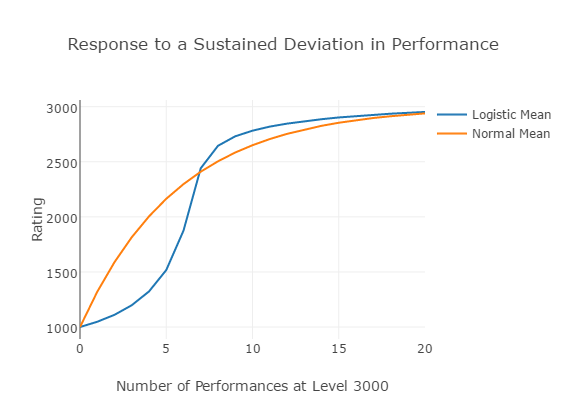
\includegraphics[scale=0.5]{../images/ResponsePlot.png} \end{center}

Had we tried to perform outlier reduction in a memoryless fashion, we would continue to increase the rating by 48 per match, oblivious to the possibility that the player truly did experience a sudden improvement. In Elo-R, the outlier status of a performance is treated as tentative. If later matches support the hypothesis of having improved, the rating will increase by an additional 63 points, followed by over 100 points in each of the third and following matches, as plotted by the blue curve above.

After six consecutive matches with $p_i = 3000$, the rating is 1875 and very unstable (even though $\sigma_i$ is unchanged!). The system is no longer sure which to trust: the extensive history at level 1000, or the smaller number of recent matches at level 3000. Depending on what comes next, the player's rating can very quickly fall toward 1000 or rise toward 3000. However, note that in either case, the change will not overshoot, say to 5000, unless enough new evidence is accumulated at that level. As the $p_i=3000$ streak continues, the seventh match on the blue curve jumps by a whopping 566 points. As the player's rating converges to 3000, the old $p_i = 1000$ data acquires outlier status, thus speeding convergence.

In contrast, while a system such as Codeforces does not compute $p_i$ values in quite in the same way, we can obtain a good approximation by removing outlier reduction from Elo-R, effectively treating the performances to be averaged as normal instead of logistic measurements. This makes the system effectively memoryless, since it turns out that each match simply moves the rating about 16\% closer to the new $p_i$ value, independent of the history. With this change, we obtain the orange curve, which jumps a whopping 320 points at the very first performance. Indeed, there is no limit: if you could find players whose ratings are extremely high, and beat them even once, your rating would take arbitrarily large leaps.

Note that this is not quite true of TopCoder, which incorporates a hack that caps the maximum rating change: if TopCoder's update formula demands too large a change, the cap kicks in. In contrast, Elo-R's cap is a natural and smooth consequence of its update formula and is sensitive to whether a change is charting new territory, or merely confirming a plausible hypothesis. TopCoder does attempt to make the magnitude of its updates sensitive to the amount of fluctuation in a player's history, using a volatility measure, but this measure does not account for the direction of the changes, resulting in the non-monotonicity flaw mentioned above.

Notwithstanding arguments that a high rating ought to properly be earned over multiple matches rather than a single fluke, the other danger is that these observations also hold in reverse: one bad day on Codeforces can seriously damage one's rating and negate several rounds of steady progress. By using heavy-tailed logistic distributions everywhere, Elo-R understands that unusually high or low performances do occasionally occur, and one round in isolation is never a reliable signal.

Interestingly, despite the slow start, the blue curve ultimately converges faster than the orange one. Since Elo-R uses its memory to dynamically adapt its view of potential outliers, it overtakes the orange curve as soon as new evidence outweighs the old hypothesis!

\subsection{Numerical analysis}

The ratings accumulate $O(\epsilon)$ numerical error per match, and likely a lot less in the long run due to statistical averaging...

\section{Conclusions}
This paper introduces the Elo-MMR rating system, which is in part a generalization of the two-player Glicko system, allowing any number of players. By developing a Bayesian model and taking the limit as the number of participants goes to infinity, we obtained simple, human-interpretable rating update formulas. Furthermore, we saw that the algorithm is incentive-compatible, robust to extreme performances, asymptotically fast, and embarrassingly parallel. To our knowledge, our system is the first to rigorously prove all these properties in a setting with more than two individually ranked players. In terms of practical performance, we saw that it outperforms existing industry systems in both prediction accuracy and computation speed.
%In particular, we compare against the popular CodeForces, Topcoder, and TrueSkill rating systems, which are deployed on platforms with hundreds of thousands to millions of users.

This work can be extended in several directions. First, the choices we made in modeling ties, pseudodiffusions, and opponent subsampling are by no means the only possibilities consistent with our Bayesian model of skills and performances. Second, it may be possible to further improve accuracy by fitting more flexible performance and skill evolution models to application-specific data.

Another useful extension would be to team competitions. Given a performance model for teams, Elo-MMR infers each team's performance. To make this useful in settings where teams are frequently reassigned, we must model teams in terms of their individual members; unfortunately, it's not possible to precisely infer an individual's performance from team rankings alone. Therefore, it becomes necessary to condition an individual's skill on their team's performance. In the case where a team's performance is modeled as the sum of its members' independent Gaussian contributions, elementary facts about multivariate Gaussian distributions enable posterior skill inferences at the individual level. Generalizing this approach to other models remains an open challenge.

% Probably redundant: The algorithm itself is trivially parallelizable, and further speedup can be attained through a simple sub-sampling strategy. We believe there is potential to improve the performance even more, either through a more sophisticated sub-sampling strategy, interpolation, or by combining our two-phase approach with a factor graph framework similar to that of TrueSkill~\cite{HMG06, KFL01}. 

Over the past decade, online competition communities such as Codeforces have grown exponentially. As such, considerable work has gone into engineering scalable and reliable rating systems. Unfortunately, many of these systems have not been rigorously analyzed in the academic community. We hope that our paper and open-source release will open new explorations in this area.

%In addition, we invite non-technical sporting communities, such as the Spartan Race and DanceSport, to find uses of our skill estimation package.

% IMPORTANT: This conference is double blind, which (aside from anonymous authors) means that we cannot post links to our git or have acknowledgements.

%\section*{Acknowledgements}
%
%I'm grateful to Daniel Sleator and Dougal Sutherland for discussions that contributed to the inspiration and preparation of this work. In addition, I'd like to thank Mike Mirzayanov for providing a useful case study by publishing the Codeforces rating algorithm.

\bibliographystyle{ACM-Reference-Format}
\bibliography{EloR}

\end{document}
